\documentclass[12pt]{article}
\usepackage{siunitx}
\usepackage{pgfplots}
\pgfplotsset{compat=1.18} % Or adjust depending on your TeX distribution
\usepackage[utf8]{inputenc}	% Para caracteres en español
\usepackage{amsmath,amsthm,amsfonts,amssymb,amscd}
\usepackage{multirow,booktabs}
\usepackage[table]{xcolor}
\usepackage{fullpage}
\usepackage{lastpage}
\usepackage{mlmodern}
\usepackage{enumitem}
\usepackage{fancyhdr}
\usepackage{mathrsfs}
\usepackage{wrapfig}
\usepackage{setspace}
\usepackage{calc}
\usepackage{multicol}
\usepackage{cancel}
\usepackage[retainorgcmds]{IEEEtrantools}
\usepackage[margin=3cm]{geometry}
\usepackage{amsmath}
\newlength{\tabcont}
\setlength{\parindent}{0.0in}
\setlength{\parskip}{0.05in}
\usepackage{empheq}
\usepackage{framed}
\usepackage[most]{tcolorbox}
\usepackage{xcolor}
\colorlet{shadecolor}{orange!15}
\parindent 0in
\parskip 12pt
\geometry{margin=1in, headsep=0.25in}
\theoremstyle{definition}
\newtheorem{defn}{Definition}
\newtheorem{reg}{Rule}
\newtheorem{exer}{Exercise}
\newtheorem{note}{Note}
\newtheorem{theorem}{Theorem}
\setcounter{section}{0}
\usepackage{chngcntr}
\usepackage{hyperref}
\counterwithin*{equation}{section}
\counterwithin*{equation}{subsection}
\usetikzlibrary{angles,quotes,calc,positioning}
\usetikzlibrary{decorations.pathmorphing, patterns, calc}

\begin{document}

\section{Guía 1}

\begin{shaded}
    \textbf{(1)} Considerar la siguiente función de movimiento de un cuerpo que se desplaza en línea recta:
\[
x(t) = 1 \, [\tfrac{m}{s^2}] \, t^2 - 3 \, [\tfrac{m}{s}] \, t
\]
donde $x$ está dado en metros y $t$ en segundos.

\begin{itemize}
    \item[(a)] Graficar la función $x(t)$.
    \item[(b)] Determinar analíticamente en todos los casos y gráficamente en los siete primeros casos, los valores de velocidad media del móvil en los siguientes intervalos de tiempo (expresados en segundos): 

\begin{align*}
    &[-1, 5], \qquad [-1, 4], \qquad [-1, 1], \qquad [-1, -0.5], \\ 
    &[-1, -0.8], \qquad [-1, -0.9], [-1, -0.99], \\ 
    &[-1, -0.999], \; [-1, -0.9999].
\end{align*}

    \item[(c)] Sea $\Delta t_n = t_n - t_0$, con $t_0 = -1 \, s$, $t_1 = 5 \, s$, $t_2 = 4 \, s$, \ldots, $t_9 = -0.9999 \, s$. A medida que $t_n$ se hace más pequeño, ¿a qué valor se aproxima la velocidad media del móvil en el intervalo $[-1, -1 + \Delta t_n]$? ¿Cómo se interpreta geométricamente este resultado?
    \item[(d)] Encuentre la ecuación de la recta tangente a la función $x(t)$ en $t = -1 \, s$.
\end{itemize}
\end{shaded}

$(a)$ Graficar una función, primer año, no es necesario hacerlo. 

$(b)$ La velocidad media de un objeto en un intervalo de tiempo de longitud
$\Delta t$ se define como $\overline{v} = \Delta x / \Delta t$. Es fácil ver que
para la lista de intervalos que nos dieron, las velocidades medias son

\begin{equation*}
    1,\quad 0,\qquad -3,\qquad -4.5,\qquad -4.8,\qquad -4.9,\qquad -4.99,\qquad -4.999
\end{equation*}

$(c)$ Veamos que

\begin{align*}
    &\lim_{\Delta t \to 0} \frac{x(-1 + \Delta t) - x(-1)}{\Delta t} =
    \frac{dx}{dt}(-1)
\end{align*}

Es decir, el límite que nos interesa es la derivada evaluada en $-1$. Como 
$x'(t) = 2t - 3$, tenemos $2(-1) - 3 = -5$, lo cual coincide con lo que
observamos en $(b)$.

$(d)$ La recta tangente a $x(t)$ en un punto $(t_0, x(t_0))$ es la única recta
que atraviesa dicho punto y cuya
pendiente es la derivada de $x(t)$ en $t_0$. La pendiente en $t_0 = -1\text{s}$,
como ya vimos, es $a = -5$. Con lo cual sólo queda determinar $b \in \mathbb{R}$
tal que $\ell(t) = -5t + b$ satisfaga $\ell(-1) = x(-1) = 4$. Resolviendo: 

\begin{equation*}
    \ell(-1) = 4 \iff -5(-1) + b = 4 \iff b = -1
\end{equation*}

La recta deseada es $\ell(t) = -5t - 1$.

\pagebreak 

\begin{shaded}
    
\textbf{(2)} Considere la posición de un móvil que se desplaza en línea recta
bajo la ecuación $x(t)$ dibujada abajo, donde $\left[ x \right] = \text{m},
x(t=0) = -3\text{m}$.

$(a)$ Determinar la longitud total del camino recorrido en $I_0 = [-1, -0.8],
I_1=[-0.6, 0.6], I_2 = [-1, 1]$. 

$(b)$ Determinar la velocidad media en dichos intervalos.
 
$(c)$ Determinar gráficamente la velocidad instantánea del móvil en los
siguientes instantes: $t = 0, t  = 0.8$.

$(d)$ Determinar aproximadamente para qué valores de $t$ el móvil se encuentra a
$1$m de distanca de la posición que tiene en $t = 0$.

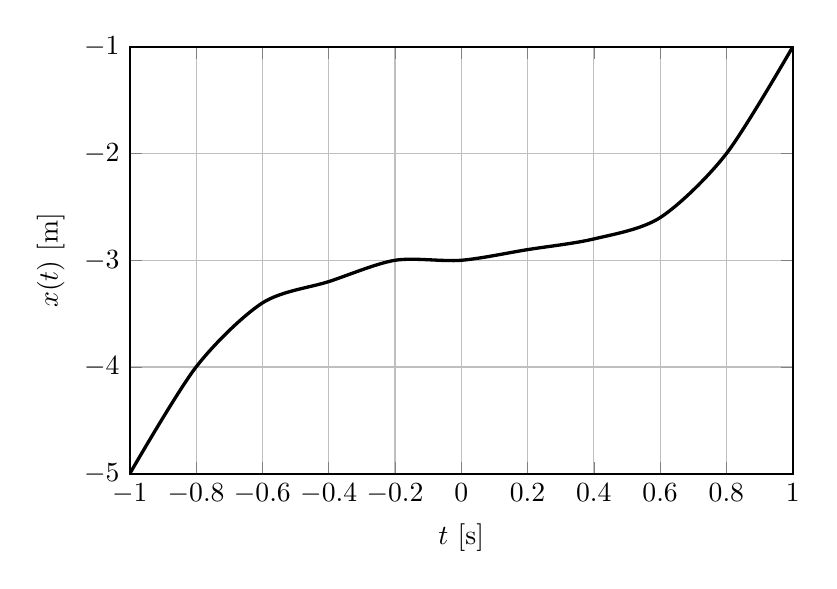
\begin{tikzpicture}
  \begin{axis}[
    width=10cm,
    height=7cm,
    grid=both,
    xlabel={$t$ [s]},
    ylabel={$x(t)$ [m]},
    thick,
    xmin=-1, xmax=1,
    ymin=-5, ymax=-1,
    ]
    % Example plot points (replace with your data or function)
    \addplot[black, very thick, smooth] coordinates {
      (-1.0,-5.0)
      (-0.8,-4.0)
      (-0.6,-3.4)
      (-0.4,-3.2)
      (-0.2,-3.0)
      (0.0,-3.0)
      (0.2,-2.9)
      (0.4,-2.8)
      (0.6,-2.6)
      (0.8,-2.0)
      (1.0,-1.0)
    };
  \end{axis}
\end{tikzpicture}
\end{shaded}

$(a)$ En el intervalo de tiempo $I_0$, el móvil se movió de la posición
$-5\text{m}$ a $-4\text{m}$, i.e. recorrió un metro. Etc. 

$(b)$ Ya sabemos hacer esto: $\overline{v} = \Delta x / \Delta t$. Etc. 

$(c)$ La velocidad instantánea en un punto $t_0$ se calcula gráficamente
dibujando la recta tangente a $x(t_0)$ y determinando la pendiente de dicha
recta. 

$(d)$ Gráficamente, se ve que se da en $t = 0.8, t = -0.8$.

\pagebreak 

\begin{shaded}
    \textbf{(5)} Sea $x(t) = -5t^2 + 17t + 3$ la función de posición de una
    partícula con $\left[ x \right] = \text{m}, \left[ t \right] = \text{s} $. 

    $(a)$ Determinar la posición de la partícula en $t =1,2,3\text{s}$.

    $(b)$ Determinar el tiempo en que la partícula retorna al origen.

    $(c)$ Obtenga $v(t)$ y determine la velocidad instantánea en
    $t=1,2,3\text{s}$, cuándo la velocidad es nula, y cuál es la velocidad de la
    partícula cuando pasa por el origen. 

    $(d)$ Grafique $x(t), v(t), a(t)$.
\end{shaded}

$(a)$ Una pavada, evaluar $x(t)$ en esos valores. 

$(b)$ La partícula retorna al origen siempre que $x(t) = 0$, con soluciones 

\begin{equation*}
    t = \frac{-17 \pm \sqrt{17^2 - 4 \cdot (-5) \cdot 3} }{-10} \iff t \in
    \left\{ -0.16815416922, 3.56815416923 \right\} 
\end{equation*}

Pero el tiempo no puede ser positivo, con lo cual la única solución que
consideramos es $t_0 \approx 3.568$.

$(c)$ $v(t) = x'(t) = -10t + 17$. La velocidad en los tiempos dados se obtiene
evaluando la función (trivial). La velocidada es nula si y solo si 

\begin{equation*}
    v(t) = 0 \iff t = \frac{17}{10} \iff t = 1.7
\end{equation*}

La velocidad al pasar por el origen es $v(t_0) \approx v(3.568) = -18.68$.

$(d)$ $a(t) = v'(t) = -10$ es una función constante. $v(t)$ es lineal y fácil de
calcular. De $x(t)$ ya conocemos las raíces, sabemos que tiene "alas" hacia
abajo (pues el coeficiente $a$ de la cuadrática es negativo), y que el máximo es
el punto medio entre las raíces, i.e. 

\begin{equation*}
    t_{\text{max}} =  \frac{ -0.16815416922 + 3.56815416923 }{2} = \frac{3.4}{2}
    = 1.7
\end{equation*}

Esto es suficiente para hacer un gráfico aproximado. Podemos agregar que $x(0) =
3$ si queremos ser más bonitos aún.

\pagebreak 

\begin{shaded}
    \textbf{6.} La figura muestra la velocidad de un móvil en función del tiempo:

\begin{center}
\begin{tikzpicture}
\begin{axis}[
    axis lines=middle,
    xlabel={$t \; [s]$},
    ylabel={$v \; [km/s]$},
    xmin=0, xmax=16,
    ymin=0, ymax=50,
    xtick={0,2,6,9,15},
    ytick={0,20,44},
    width=12cm,
    height=7cm,
    samples=200,
    domain=0:15,
]
\addplot[thick,black] coordinates {
    (0,20) (6,20) (9,44) (15,0)
};
\end{axis}
\end{tikzpicture}
\end{center}

\begin{enumerate}
    \item[(a)] Determine la aceleración instantánea del móvil para $t=3\,s$ y $t=11\,s$.
    \item[(b)] Calcule la distancia recorrida por el móvil en los intervalos de tiempo $t=[0,5]\,s$, $t=[0,9]\,s$ y $t=[0,15]\,s$.
    \item[(c)] Conociendo que $x(t=6\,s)=0\,m$, encuentre la posición del móvil en $t=0\,s$.
    \item[(d)] Dé una expresión de la posición del móvil válida para todo $t$.
    \item[(e)] Grafique $x(t)$, $v(t)$ y $a(t)$.
\end{enumerate}
\end{shaded}

$(a)$ Del gráfico obtenemos que 

\begin{equation*}
    v(t) = \begin{cases}
        20 & 0 \leq t < 6\\ 
        \ell_1(t) &6 \leq t < 9 \\ 
        \ell_2(t) &9\leq t \leq 15
    \end{cases}
\end{equation*}

donde $\ell_1, \ell_2$ son funciones lineales a determinar. Sabemos que
$\ell_1(6) = 20, \ell_1(9) = 44$, lo cual es suficiente para determinar la
función. La pendiente es

\begin{equation*}
    a_1 = \frac{\Delta \ell_1}{\Delta t} = \frac{44 - 20}{9 - 6} = 8
\end{equation*}

Como $\ell_1(6) = 20$, necesitamos $8\cdot 6 + b_1 = 20 \iff b_1 = -28$. 

$\therefore $ $\ell_1(t) = 8t - 28$.

De manera análoga se determina que $\ell_2(t) = - \frac{22}{3}t + 110$.

Sabiendo $v(t)$, determinamos la aceleración como 

\begin{equation*}
    a(t) = v'(t) = \begin{cases}
        0 & 0 \leq t < 6 \\ 
        8 & 6 \leq t < 9 \\ 
        -\frac{22}{3} & 9 \leq t \leq 15
    \end{cases}
\end{equation*}

lo cual es suficiente para calcular la aceleración instantánea en los puntos de
interés.

$(b)$ La distancia recorrida por un móvil con función de velocidad $v(t)$ en un
intervalo de tiempo $I$ es 

\begin{equation*}
    \int_I \left| v(t) \right| ~ dt
\end{equation*}

Para un intervalo general $I = [a, b]$, usando el hecho de que $v(t) > 0
\Rightarrow \left| v(t) \right| = v(t)$,

\begin{equation}
    \int_I \left| v(t) \right| ~ dt 
    &= x(b) - x(a)
\end{equation}

pues $x(t)$ es la primitiva de $v(t)$. Pero 

\begin{align*}
    x(t) 
    &= \int v(t) ~ dt \\ 
    &=\begin{cases}
        20t + \varphi_1 & 0 \leq t < 6 \\ 
        4t^2 - 28t + \varphi_2 & 6 \leq t < 9 \\ 
        -\frac{22}{6}t^2 + 110t + \varphi_3 & 9 \leq t \leq 15
    \end{cases}
\end{align*}

para algunas constantes $\varphi_1,  \varphi_2, \varphi_3 \in \mathbb{R}$.
Dichas constantes dependen del sistema de coordenadas elegido para la función de
posición, pero además deben satisfacer las restricciones de continuidad. Sabemos
que $x(6) = 0$ por el enunciado $(c)$. Entonces $x(6) = 20t + \varphi_1 = 0 \iff
\varphi_1 = -120$. Para satisfacer continuidad, necesitamos 

\begin{equation*}
    20(6) - 120 = 4(6^2) - 28(6) + \varphi_2 \iff \varphi_2 = 24
\end{equation*}

De manera análoga se obtiene $\varphi_3= -597$. Por lo tanto, 

\begin{equation*}
    x(t) = \begin{cases}
        20t - 120 & 0 \leq t < 6 \\ 
        4t^2 -28t  + 24 & 6 \leq t < 9 \\ 
        -\frac{22}{6}t^2 + 110t -597 & 9 \leq t \leq 15
    \end{cases}
\end{equation*}

Usando la ecuación $(1)$, la distancia recorrida en $I_0 = [0, 5]$ será 

\begin{equation*}
    x(5) - x(0) = -20 + 120 = 100
\end{equation*}

(en kilómetros). Para $I_1 = [0, 9]$ será 

\begin{equation*}
    \int_0^6 v(t) ~ dt + \int_6^9 v(t) ~ dt = \left[ x(6) - x(0) \right] +
    \left[ x(9) - x(6) \right] = \text{etc.}
\end{equation*}

$(d)$ Ya lo hicimos al hallar $x(t)$. 

$(e)$ Etc.

\pagebreak 

\begin{shaded}
    \textbf{(7)} Un camión y un auto parten en el instante $t=0$, el auto
    estando cierta distancia $\Delta x$ tras el camión. El camión  tiene una
    aceleración $a_{\text{truck}} = 1.2\text{m/s}^2$, el auto una aceleración
    $a_{\text{car}} = 1.8\text{m/s}^2$. El auto alcanza al camión cuando éste ha
    recorrido 45m. 

    $(a)$ Determinar el tiempo $t_*$ que tarda el auto en alcanzar al camión.

    $(b)$ Determinar $\Delta x$. 

    $(c)$ Determinar $v_{\text{car}}(t_*), v_{\text{truck}}(t_*)$.

    $(d)$ Graficar posición, velocidad y aceleración de ambos.
\end{shaded}

$(a)$ Sabiendo las aceleraciones, podemos determinar las velocidades y con ellas
las posiciones. En particular, 

\begin{align*}
    &v_{\text{car}}(t) = 1.8 t \text{ m/s} + \alpha_1 \text{ m/s}, \qquad x_{\text{car}}(t) =
    0.9t^2 + \alpha_1 t \text{ m} + \alpha_2\text{ m}\\ 
    &v_{\text{truck}}(t) = 1.2\text{ m/s} + \beta_1\text{ m/s},\qquad x_{\text{truck}}(t) =
    0.6t^2\text{ m} + \beta_1 t \text{ m} + \beta_2 \text{ m}
\end{align*}

con $\alpha_i, \beta_i \in \mathbb{R}$ para $i=1,2$. Ambos vehículos
parten en el instante $t=0$, así que en dicho instante sus velocidades son
nulas:

\begin{equation*}
    v_{\text{car}}(t=0) = 0 \Rightarrow \alpha_1 =0, \qquad
    v_{\text{truck}}(t=0) = 0 \Rightarrow \beta_1 = 0
\end{equation*}

Si definimos el origen de nuestro sistema como el punto de partida del auto,

\begin{align*}
    x_{\text{car}}(t=0) = 0 \Rightarrow  \alpha_2 = 0, \qquad
    x_{\text{truck}}(t=0) =  \Delta x \Rightarrow \beta_2 = \Delta x
\end{align*}

Por lo tanto,

\begin{align*}
    &v_{\text{car}}(t) = 1.8 t \text{ m/s}, \qquad x_{\text{car}}(t) =
    0.9t^2, \\
    &v_{\text{truck}}(t) = 1.2\text{ m/s}, \qquad x_{\text{truck}}(t) =
    0.6t^2\text{ m} + \Delta x\text{ m}
\end{align*}

El instante $t_*$ es el instante en que el camión ha recorrido 45m:


\begin{align*}
    \int_0^{t_*} v_{\text{truck}}(t) ~ dt = 45 \iff 
    &x_{\text{truck}}(t_*) - x_{\text{truck}}(0) = 45 \\ 
    \iff ~ ~ ~ 
    &0.6t_*^2 + \Delta x - \Delta x = 45 \\ 
    \iff  ~ ~  ~ 
    &0.6t_*^2 = 45 \\ 
    \iff ~ ~ ~ 
    &t_*^2 = 75 \\ 
    \iff ~ ~ ~ 
    &t_* = 5\sqrt_*{3}  
\end{align*}

$(b)$ Sabemos que $x_{\text{car}}(t_*) = x_{\text{truck}}(t_*)$, con lo cual
obtenemos 

\begin{equation*}
    0.9(5\sqrt{3} )^2 = 0.6(5\sqrt{3} )^2 + \Delta x \iff \Delta x = 22.5
\end{equation*}

$(c)$ Una pavada. 

$(d)$ Una pavada.

\pagebreak 

\begin{shaded}
    \textbf{(8)} Un automóvil se desplaza por una carretera que es paralela a la vía de un tren. El automóvil se detiene ante un semáforo que está con luz roja en el mismo instante que pasa un tren con una velocidad constante de $12.0 \, \mathrm{m/s}$. El automóvil permanece detenido durante $6.0 \, \mathrm{s}$ y luego parte con una aceleración constante de $2.0 \, \mathrm{m/s^2}$.  

Determine:
\begin{enumerate}[(a)]
    \item El tiempo que emplea el automóvil en alcanzar al tren, medido desde el instante en que se detuvo ante el semáforo.
    \item La distancia que recorrió el automóvil desde el semáforo hasta que alcanzó al tren.
    \item La velocidad del automóvil en el instante que alcanza al tren.
\end{enumerate}
\end{shaded}

$(1)$ Sea $t = 0$ el tiempo en que el auto se detiene en el semáforo, y $x(0)$
la posición del semáforo. Sabemos que para $t \geq 6$,

\begin{equation*}
    v_{\text{car}}(t) = 2t \text{ m/s} + \alpha_1, \qquad x_{\text{car}}(t) =
    t^2 \text{ m} + \alpha_1 t + \alpha_2
\end{equation*}

siendo ambas funciones constanatemente nulas para $0 \leq t < 6$.

Como la velocidad en el instante $t=6$ es nula, $v_{\text{car}}(6) = 0 \iff 12 +
\alpha_1 = 0 \iff \alpha_1 = -12$. Como la posición en el instante 6 es nula,
$6^2 -12(6) + \alpha_2 = 0 \iff \alpha_2 = 36$.

\begin{equation*}
    \therefore \qquad v_{\text{car}}(t) = 2t \text{ m/s} - 12\text{ m/s}, \qquad x_{\text{car}}(t) =
    t^2 \text{ m} -12t \text{ m} + 36\text{ m}
\end{equation*}

para $t \geq 6$. De manera análoga, para todo $t \geq 0$,

\begin{equation*}
    x_{\text{train}}(t) = 12t  \text{ m}
\end{equation*}

donde la constante de integración debe ser cero para satisfacer que la posición
del tren en el instante inicial es nula.

El tiempo $t_* > 6$ en que el auto alcanza al tren satisface 

\begin{align*}
x_{\text{train}}(t_*)
= x_{\text{car}}(t_*) 
\iff 
&12t_* = t_*^2 -12 t_* + 36\\ 
\iff
&t_*^2 -24t_* + 36 = 0
\end{align*}

con soluciones 

\begin{equation*}
    t_* = \frac{24 \pm \sqrt{24^2 -4 (36)} }{2} \iff t_* \in \left\{
    1.60769515459, 22.3923048454 \right\} 
\end{equation*}

La solución $t_* \approx 1.608$ no debe considerarse y por ende $t_* \approx
22.392$.

$(2)$ La distancia recorrida por el automóvil desde el semáforo hasta que
alcanzó el tren es dada por 

\begin{align*}
    \int_{t=0\text{s}}^{t=t_*\text{s}} \left| v_{\text{car}}(t) \right| ~ dt 
    &= \int_{t=6\text{s}}^{t={t_* \text{s}}} \left| v(t) \right| ~dt \\
    &= \int_{t=6\text{s}}^{t={t_* \text{s}}}  v(t) ~dt \\ 
    &=x(t_*) - x(6)\\ 
    &=x(t_*)
\end{align*}

donde el valor absoluto desaparece puesto que en $t \geq 6$ la función integrada
es claramente mayor o igual a cero. Usando la aproximación $t_* \approx 22.392$,
se obtiene $x(t_*) \approx 268.697 \text{ m}$.

$(c)$ Una pavada: evaluar $v_{\text{car}}(t_*)$.

\pagebreak 

\begin{shaded}
    \textbf{(11)} El movimiento en el plano de una partícula es dado por 
    $x(t) = at^2$ e $y(t) = bt^3$ con $a = 3 \text{m/s}^2, b = 2\text{m/s}^3$.

    $(a)$ Hallar la trayectoria de la particula. 

    $(b)$ Calcular su aceleración en $t = 12$s. 

    $(c)$ Calcular el ángulo entre los vectores velocidad y aceleración en dicho
    instante. 

    $(d)$ Determinar el instante $t_1$ en que la aceleración es paralela a la
    recta $y = x$ y el instante $t_2$ en que la velocidad lo es. 

    $(e)$ Determinar la velocidad media entre los dos instantes calculados en
    $(d)$.
\end{shaded}


$(a)$ La trayectoria es el conjunto de puntos 

\begin{align*}
    S 
    &= \left\{ \left( x(t),  y(t) \right) : t \in \mathbb{R}  \right\} \\ 
    &= \left\{ (at^2, bt^3) : t \in \mathbb{R}\right\} 
\end{align*}

Dado un punto $p_0 = (x, y)$ arbitrario de la trayectoria, se satisface que 

\begin{equation*}
    x = at^2, \qquad y = bt^3
\end{equation*}

Tomemos $t \geq 0$. De la primera ecuación deducimos $t =
\sqrt{\frac{x}{a}} $. De la segunda ecuación deducimos 

\begin{equation*}
    y = bt^3 = b \left( \frac{x}{a}
    \right)^{\frac{3}{2}}
\end{equation*}

Por lo tanto, para todo $t \geq 0$, la función 

\begin{equation*}
    \tau(x) = b\left( \frac{x}{a} \right)^{\frac{3}{2}}
\end{equation*}

describe la trayectoria del móvil.

$(b)$ La velocidad y aceleración del móvil es dada por

\begin{equation*}
    v_x(t) = 2at, \qquad a_x(t) = 2a, \qquad \qquad v_y(t) = 3bt^2, \qquad
    a_y(t) = 6bt
\end{equation*}

o más rigurosamente 

\begin{equation*}
    v(t) = 6t \hat{i} + 6t^2 \hat{j}, \qquad a(t) = 6 \hat{i} + 12t \hat{j}
\end{equation*}

La aceleración en $t = 12$ es trivial: evaluar $a(t)$ en dicho valor.


$(c)$ A calcularla nomás: 

\begin{equation*}
    v(12) = 72 \hat{i} + 864 \hat{j}, \qquad \qquad
    a(12) =  6 \hat{i} + 144 \hat{j}
\end{equation*}

donde la unidad de la coordenada $x$ está en $\text{m/s}^2$, y la de $y$ en
$\text{m/s}^3$. Recordemos que el producto punto entre dos vectores se define 
como

\begin{equation*}
    \vec{w} \cdot \vec{u} = uw \cos \theta
\end{equation*}

con $\cos \theta$ el ángulo entre ellos, pero que además satisface que 
$\vec{w} \cdot \vec{u} = \vec{w}_x \vec{u}_x + \vec{w}_y \vec{u}_y$. Por ende,
el producto cruz de los vectores de aceleración y posición satisface 

\begin{align*}
    72(6) + 864(144) = \left| v(12) \right| \left| a(12) \right|
    \cos \theta
\end{align*}

Las magnitudes de ambos vectores son 

\begin{equation*}
    \left| v(12) \right| = 866.995, \qquad \left| a(12)
    \right| = 144.125
\end{equation*}

Sustituyendo con el resultado de las operaciones y dividiendo por el producto de
las magnitudes, obtenemos

\begin{equation*}
    0.99827265479 = \cos \theta \iff \theta = 1.51201125\text{rad}
\end{equation*}

$(d)$ Queremos saber el instante $t_1$ en que el ángulo $\varphi$ entre la
aceleración y la recta $y = x$ es nulo, i.e. el momento en que el ángulo entre
la aceleración y el eje $x$ es $\frac{\pi}{4}$. Hay dos formas de resolver esto.
La más simple es ver que el vector tiene dicho ángulo si y solo si la componente
$x$ es igual a la componente $y$, y planteando al ecuación 

\begin{equation*}
    a_x(t_1) = a_y(t_1) \iff 6 = 12t_1 \iff t_1 = 1 / 2
\end{equation*}

Sólo para tener en cuenta que nos podrían haber pedido un ángulo $\varphi$ menos
obvio respecto al eje $x$, la forma general (pero más densa) de calcular esto
es planteando la ecuación:

\begin{align*}
    &\frac{ \vec{a}(t_1) \cdot \hat{i} }{\left| \vec{a}(t_1) \right| \left|
    \hat{i} \right| } = \cos \varphi \\
    \iff ~ ~ ~ 
    &\frac{a_x(t_1)}{\left| \vec{a}(t_1)
\right| } = \cos(\frac{\pi}{4}) \\ 
\iff ~ ~ ~ 
    &\frac{6}{\sqrt{6^2 + 12^2t_1^2} } = 
\frac{ \sqrt{2}  }{2} \\ 
\iff ~ ~ ~ 
    &\frac{ 36 }{36 + 144t_1^2} = \frac{1}{2}\\ 
    \iff ~ ~ ~ 
    &72 = 36 + 144t_1^2\\
    \iff ~ ~ ~ 
    &144t_1^2 -36 = 0 \\ 
    \iff ~ ~ ~ 
    &36\left( 4t_1^2 - 1 \right) =0 \\ 
    \iff ~ ~ ~ 
    &4t_1^2 - 1 = 0\\
    \iff ~ ~ ~ 
    &4t_1^2 = 1\\
    \iff ~ ~ ~ 
    &t_1^2 = \frac{1}{4}
\end{align*}

Como $t > 0$ esto da una única solución $t_1 = 1 / 2$. Para la velocidad hacemos
solo la forma simple, viendo que 

\begin{equation*}
    v_x(t_2) = v_y(t_2) \iff 6t_2 = 6t_2^2 \iff t_2 = t_2^2 \iff t = 1
\end{equation*}

(pues $t > 0$).  

$(e)$ La velocidad media entre los dos instantes es 


\begin{equation*}
    \Delta \vec{x} / \Delta t = \frac{(3 * 1^2 - 3*( 0.5^2 ), 2*1^3 -
    2*(0.5^2)}{0.5} = \frac{(2.25, 1.75)}{0.5} = (4.5, 3.5)\text{m/s}
\end{equation*}




















































\end{document}



